\documentclass[3pt,landscape]{article}
%ss[10pt,landscape]{article}
\usepackage{multicol}
\usepackage{calc}
\usepackage{ifthen}
\usepackage[landscape]{geometry}
\usepackage{amsmath,amsthm,amsfonts,amssymb}
\usepackage{color,graphicx,overpic}
\usepackage{hyperref}


\pdfinfo{
/Title (example.pdf)
/Creator (TeX)
/Producer (pdfTeX 1.40.0)
/Author (Seamus)
/Subject (Example)
/Keywords (pdflatex, latex,pdftex,tex)}

% This sets page margins to .5 inch if using letter paper, and to 1cm
% if using A4 paper. (This probably isn't strictly necessary.)
% If using another size paper, use default 1cm margins.
\ifthenelse{\lengthtest { \paperwidth = 11in}}
    { \geometry{top=.5in,left=.5in,right=.5in,bottom=.5in} }
    {\ifthenelse{ \lengthtest{ \paperwidth = 297mm}}
        {\geometry{top=1cm,left=1cm,right=1cm,bottom=1cm} }
        {\geometry{top=1cm,left=1cm,right=1cm,bottom=1cm} }
    }

% Turn off header and footer
\pagestyle{empty}

% Redefine section commands to use less space
\makeatletter
\renewcommand{\section}{\@startsection{section}{1}{0mm}%
                            {-1ex plus -.5ex minus -.2ex}%
                            {0.5ex plus .2ex}%x
                            {\normalfont\large\bfseries}}
\renewcommand{\subsection}{\@startsection{subsection}{2}{0mm}%
                            {-1explus -.5ex minus -.2ex}%
                            {0.5ex plus .2ex}%
                            {\normalfont\normalsize\bfseries}}
\renewcommand{\subsubsection}{\@startsection{subsubsection}{3}{0mm}%
                            {-1ex plus -.5ex minus -.2ex}%
                            {1ex plus .2ex}%
                            {\normalfont\small\bfseries}}
\makeatother

% Define BibTeX command
\def\BibTeX{{\rm B\kern-.05em{\sc i\kern-.025em b}\kern-.08em
    T\kern-.1667em\lower.7ex\hbox{E}\kern-.125emX}}

% Don't print section numbers
\setcounter{secnumdepth}{0}


\setlength{\parindent}{0pt}
\setlength{\parskip}{0pt plus 0.5ex}

%My Environments
\newtheorem{example}[section]{Example}
% -----------------------------------------------------------------------

\def\ci{\perp\!\!\!\perp}

\begin{document}
\raggedright
\footnotesize
\begin{multicols}{3}


% multicol parameters
% These lengths are set only within the two main columns
%\setlength{\columnseprule}{0.25pt}
\setlength{\premulticols}{1pt}
\setlength{\postmulticols}{1pt}
\setlength{\multicolsep}{1pt}
\setlength{\columnsep}{2pt}

\begin{center}
    \Large{\underline{CS 161 Final Cheat Sheet}} \\
\end{center}

\subsubsection*{Kerchoff's Principle}
You should not rely on the secrecy of the algorithm/protocol and or keysize, as wall as the possible plain text for security because eventually the adversary will figure them out.

\subsubsection*{Mono-Alphabetic Ciphers: 1 to 1 mapping of characters to symbols}
\begin{itemize}
    \item Subsitution
        \begin{itemize}
            \item Shift or Caesar's Cipher
                \(E_{k}(m) \leftarrow m+k(\texttt{mod } N)\)
                \(D_{k}(c) \leftarrow c-k(\texttt{mod } N)\)
            \item Affine Cipher:
                \(E_{k}(m) \leftarrow k_{!}m+k_{2}(\texttt{mod } N)\)
                \(D_{k}(c) \leftarrow k_{!}^{-1}(c-k(\texttt{mod } N)\)
            \item Substitution Ciphers have an extreme vulnerability to frequency attacks.
        \end{itemize}
\end{itemize}

\subsubsection*{Poly-Alphabetic Ciphers}
\begin{itemize}
    \item Vigenere Cipher: Shift by a repeated key
    \item Book Cipher (Beale Cipher) key is hidded in a passage of a set book.
    \item Vernam Cipher
        \begin{itemize}
            \item Message is m bits and the key is n bits.
            \item Bitwise xor the message and the key, if m is greater than n, then use the key multiple times.
        \end{itemize}
    \item One-Time Pad
        \begin{itemize}
            \item Same idea as the Vernam Cipher except we use a key that is the same length or greater than the length of the message, then discard it after each use.
        \end{itemize}
    \item Transposition/Permutation Cipher
        \begin{itemize}
            \item Break the message into n bit blocks, then on each block perfom the same permutation
            \item Despite being polyalphabit, the cipher is still vulnerable to frequency attacks. Because the original patterns are still basically present. You can attack by checking anagrams.
        \end{itemize}
\end{itemize}

\subsection*{Data Encryption Standard (DES)}
DES is a block cipher in which messages are divided into data blocks of a fixed length and each block is treated as one message either in M or in C. The DES encryping and decryption algorithms take as an input a 64-bit plaintext or ciphertext message and a 56-bit key, and output a 64-bit ciphertext or plaintext message.
DES is done in 3 steps:
\begin{enumerate}
    \item Apply a fixed "initial permutation" IP to the input block.
        \((L_0,R_0) \leftarrow IP(\texttt{Input Block})\) 
        This step has no apparent cryptographic significance.
    \item Iterate the following 16 rounds of operations (Feistel Cipher)\\
        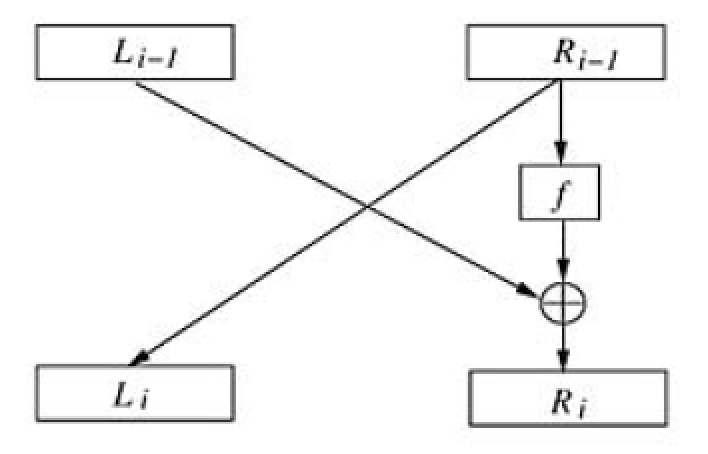
\includegraphics[scale=.47]{feistel}
        \\
        \begin{itemize}
            \item the function is nonlinear and is considered a Substitution Cipher
            \item the move from \(L_{i} \rightarrow R_{i-1}\) is a Transposition cipher
            \item Vernam cipher is used at the xor
            \item k is a 48 bit subsection of the 56 bit, "round key"
        \end{itemize}
\end{enumerate}

\subsubsection*{Single DES}
\begin{itemize}
    \item vulnerable to brute force or exaustive key search attacks
\end{itemize}

\subsubsection*{Triple DES}
Triple DES uses an encryption-decryption-encryption scheme,\\
\(c \leftarrow E_{k_{1}}(D_{k_{2}}(E_{k_{1}}(m)))\)\\
\(m \leftarrow D_{k_{1}}(E_{k_{2}}(D_{k_{1}}(m)))\)\\
This scheme enlarges the keyspace while maintaining backward compatibility with single DES if \(k_{1}=k_{2}\)

\subsection*{Advanced Encryption Standard (AES)}
AES is a block cipher with variable block size and variable keysize. (block size can be 128, 192, 256 bit)\\
AES has 4 states:
\begin{enumerate}
    \item Sub Bytes State: nonlinear substitution on each byte
    \item Shift Rows State: Transposition rearranges the order of elements in each row
    \item Mix Columns State: Polynomial multiplication after converting column to polynomial.
    \item Add Round Key State: adds elements of round key to the state, basically bitwise "OR"
\end{enumerate}
Decryption is the inverse of these steps.

\subsubsection*{Confidentiality Modes of Operation}
Different modes of operation have been devised on top of an underlying block cipher algorithm
\begin{itemize}
    \item Electronic Codebook (ECB) Mode
\end{itemize}

% You can even have references
\rule{0.3\linewidth}{0.25pt}
\scriptsize
\bibliographystyle{abstract}
\bibliography{refFile}
\end{multicols}
\end{document}
